\documentclass{article}
%\usepackage[OT4]{fontenc}
%\usepackage[polish]{babel}
\usepackage{polski}
\usepackage[utf8]{inputenc}
\usepackage{apacite}
\usepackage{natbib}
\usepackage{caption}
\usepackage{booktabs}
\usepackage{colortbl, xcolor}
\usepackage{tabularx}
\usepackage{graphicx}
\usepackage{multirow}
\usepackage{epstopdf}

\author{Michał Burdukiewicz, Przemysław Gagat}
\title{n-gramowa analiza białek metanogenów\linebreak \vskip{} 
\large{Projekt badawczy Doktoranckiego Koła Naukowego Bioinformatyki}} 
\date{}

\AtBeginDocument{%
  \renewcommand{\tablename}{Tab.}
} 

\AtBeginDocument{%
  \renewcommand{\figurename}{Rys.}
} 

\begin{document}

\maketitle

\section{Założenia projektu badawczego}

Metanogeny to zróżnicowana grupa archeonów


% latex table generated in R 3.3.1 by xtable 1.8-2 package
% Thu Jul 14 09:41:13 2016
\begin{table}[ht]
\centering
\caption{Przykładowy skrócony alfabet 
aminokwasowy. Sekwencja ADPH w tym alfabecie 
zostanie zapisana jako 1335.} 
\begin{tabular}{rl}
  \toprule
Numer grupy & Aminokwasy \\ 
  \midrule
  1 & A, G \\ 
   \rowcolor[gray]{0.85}  2 & C \\ 
    3 & D, E, K, N, P, Q, R, S, T \\ 
   \rowcolor[gray]{0.85}  4 & F, I, L, M, V, W, Y \\ 
    5 & H \\ 
   \bottomrule
\end{tabular}
\label{tab:przykladowy}
\end{table}

Nasze wstępne wyniki sugerują, że w przypadku niektórych problemów 
przewidywania właściwości białek, zastosowanie skróconego alfabetu 
aminokwasowego może znacząco ulepszyć precyzję predykcji. Jednakże taki alfabet  
musi zostać wybrany spośród wielu potencjalnych skróconych alfabetów. Liczba 
wszystkich możliwych skróconych alfabetów aminokwasowych $n_s$ zawierających $k$ 
grup jest wyrażona poprzez: 

$$ n_s = \frac{1}{k!} \sum^{k}_{j = 0} (-1)^{k-j}  {k \choose j} j^{20} $$

Nawet przy założeniu, że optymalna wielkość skróconego alfabetu jest już znana, 
to liczba potencjalnych możliwości jest bardzo duża (np. wszystkich alfabetów 
sześcioelementowych jest $4.306079 \times 10^{12}$).

\section{Obecny stan badań}

Baza Methanogenes jest największym zbiorem informacji na temat 
metanogenów. Jej zaletą, oprócz kompletności zgromadzonych danych, są 
narzędzia wizualizacyjne pozwalające na interaktywne porównywanie ze 
sobą różnych metanogenów pod względem ich cech fenotypowych.

Jakkolwiek istniejące funkcje wizualizacyjne są bardzo pomocne, to obecnie brak 
narzędzi umożliwiających jednoczesną wizualizację więcej niż dwóch zmiennych. 
To ograniczenie wydaje się szczególnie doktliwe biorąc pod uwagę ogrom 
informacji zgromadzonych w bazie Methanogenes. 

Istotnym brakiem bazy Methanogenes jest nieobecność w niej sekwencji 
nukleinowych i aminokwasowych metanogenów. Taka informacja jest cenna we 
wszelkiego rodzaju metodach biologii obliczeniowej, w tym 
badaniach filogenetycznych. Wzbogacenie bazy metanogenów o odpowiednie 
sekwencje nukleinowe i aminokwasowe z pewnością uczyni ją przydatniejszą dla 
szerszego grona użytkowników pod warunkiem dodania do bazy oprogramowania 
umożliwiające efektywne przeszukiwanie zbioru sekwencji.

Sekwencje poszczególnych gatunków metanogenów mogą zostać graficznie opisane za 
pomocą częstości pojedynczych reszt, aminokwasów lub nukleotydow. Tego rodzaju 
dane można wykorzystać do analizy skupień lub skonfrontować je z informacjami 
fenotypowymi, już obecnymi w bazie.

\section{Cel badań}

Głównym zadaniem badawczym jest opracowanie nowych metod wizualizacji danych w 
bazie Methanogenes. Ponieważ baza nie zawiera jeszcze wielu informacji 
istotnych z punktu widzenia biologii obliczeniowej, zostaną one dodane w 
trakcie trwania projektu.

\section{Metody}

\subsection{Pozyskanie i przeszukiwanie sekwencji metanogenów}

Sekwencje nukleotydowe i aminokwasowe metanogenów zostaną pozyskane z baz NCBI, 
odpowiednio Nucletide i Protein. W celu automatyzacji procesu, sekwencje 
zamiast ręcznie zostaną pozyskane z użyciem EUtils API udostępnionym przez NCBI 
(\url{http://www.ncbi.nlm.nih.gov/books/NBK25500/}).

W celu zagwarantowanie większej jakości pozyskanych rekordów, sekwencje zostaną 
poddane ręcznej kuracji. 

Zgromadzony zbiór sekwencji będzie można przeszukiwać dzięki lokalnej instancji 
algorytmu Blast XXX.

\subsection{Analiza częstościowa}

DO bazy zostanie dodany web server odpowiedzialny za wizualizację sekwencji za 
pomocą analizy częstościowej. Zwyczajowa analiza występowania 
pojedynczych reszt nukletydowych lub aminokwasowych zostanie rozszerzona o 
analizę n-gramów, ciągłych lub nieciągłych podsekwencji długości $n$. 
Obliczenia zostaną wykonane dzięki narzędziom z pakietu \textit{biogram} XXX, a 
web server zostanie zrealizowany w technologii \textit{shiny}.

\subsection{Analiza skupień}

Web server dedykowany analizie skupień danych zgromadzonych w bazie zostanie 
oparty o algorytm klasteryzacji gęstościowej (Ester et al. (1996) XXX). Metodę 
tę wybraną ze względu na odporność na zaszumienie danych i szybkość działania. 
Analiza będzie w pełni interaktywna, co oznacza, że użytkownik będzie mógł 
wybrać interesujące go cechy, a następnie określić parametry działania 
algorytmu. 

Wynikiem analizy nie będą tylko dane liczbowe, ale również graficzna 
reprezentacja znalezionych klastrów.


\begin{figure}[htbp]
\centering
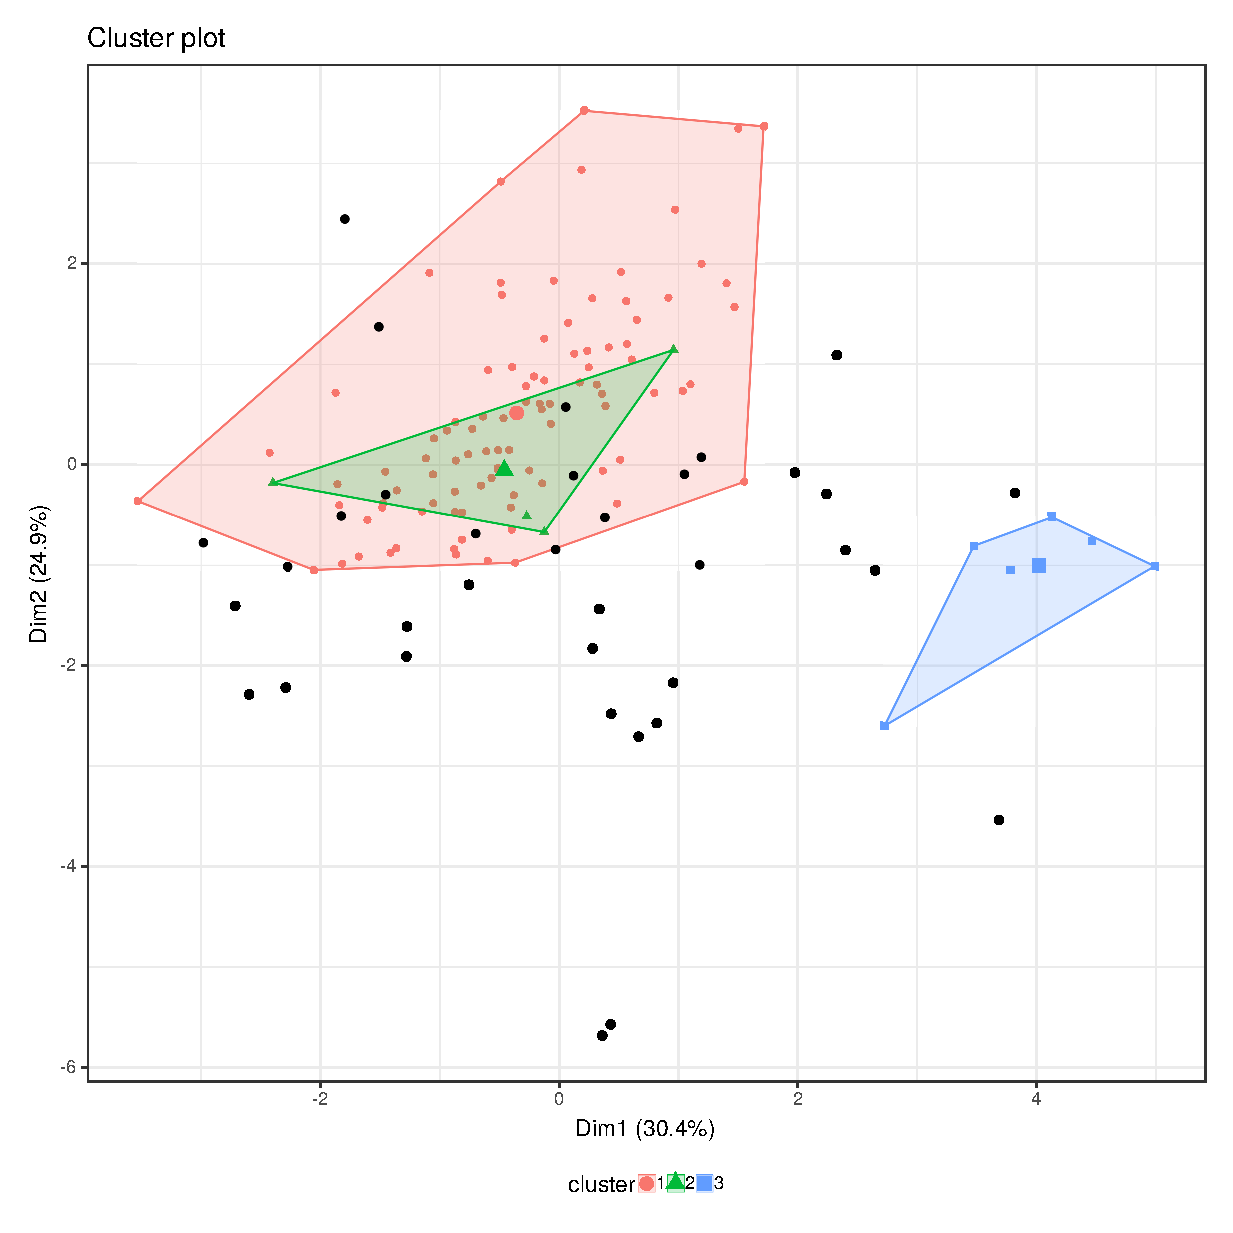
\includegraphics[width=0.9\textwidth]{cluster.eps}
\caption{Wyniki PCA dla częstości aminokwasów w peptydach sygnałowych i 
dojrzałych białkach \textit{Plasmodiidae} oraz innych eukariontów.}
\label{fig:cluster}
\end{figure}

\section{Czas realizacji projektu}

Projekt będzie realizowany w okresie 1.06.2017 do 30.11.2017.

\section{Planowane wydatki}

Łączny koszt projektu badawczego to 29 796,00 zł.

\begin{table}[!htbp]
\centering
\caption{Kosztorys projektu badawczego.}
\begin{tabular}{rrr}
\cline{1-2}
\multicolumn{1}{|c}{Nazwa}                                   & \multicolumn{1}{|c|}{Koszt}   &  \\ \cline{1-2}
\multicolumn{1}{|c}{Akcesoria niezbędne w realizacji zadań badawczych}   & 
\multicolumn{1}{|c|}{760,00 zł} &  \\ \cline{1-2}
\multicolumn{1}{|c}{Wyjazdy konferencyjne}   & 
\multicolumn{1}{|c|}{4 000,00 zł} &  \\ \cline{1-2}
Łącznie    & 29 796,00 zł                    & 
\end{tabular}
\end{table}

\subsection{Akcesoria niezbędne w realizacji zadań badawczych}

Właściwe zrealizowanie projektu badawczego wymaga również dokupienie 
akcesoriów (Tab.~\ref{tab:akcesoria}), takich jak pamięci USB niezbędne do 
przenoszenia duzych objętości danych i słuchawki z mikrofonem do prowadzenia 
rozmów z zagranicznym uczestnikiem projektu. Wykonanie części zadań badawczych 
nie byłaby możliwa gdyby nie komputery przenośne udostępnione członkom Koła 
przez Zakład Genomiki. Bezpieczny transport otrzymanego sprzętu wymaga zakupu 
specjalnych plecaków na laptopy.

\begin{table}[]
\centering
\caption{Koszty akcesoriów niezbędnych w realizacji zadań badawczych.}
\label{tab:akcesoria}
\begin{tabular}{ccccc}
\cline{1-4}
\multicolumn{1}{|c|}{Nazwa}                           & \multicolumn{1}{c|}{Cena 
(szt.)} & \multicolumn{1}{c|}{Liczba} & \multicolumn{1}{c|}{Łączna cena} &       
               \\ \cline{1-4}
\multicolumn{1}{|c|}{Pendrive USB 3.0 - 32 GB}        & 
\multicolumn{1}{c|}{45,00 zł}    & \multicolumn{1}{c|}{4}      & 
\multicolumn{1}{c|}{180,00 zł}   &                      \\ \cline{1-4}
\multicolumn{1}{|c|}{Słuchawki z mikrofonem Creative} & 
\multicolumn{1}{c|}{140,00 zł}   & \multicolumn{1}{c|}{2}      & 
\multicolumn{1}{c|}{280,00 zł}   &                      \\ \cline{1-4}
\multicolumn{1}{|c|}{Plecak na laptopa}               & 
\multicolumn{1}{c|}{150,00 zł}   & \multicolumn{1}{c|}{2}      & 
\multicolumn{1}{c|}{300,00 zł}   & \multicolumn{1}{l}{} \\ \cline{1-4}
                                                      &                          
        & Łącznie:                    & 760,00 zł                        &       
              
\end{tabular}
\end{table}

\subsection{Wyjazdy konferencyjne}

Utworzone web servery zostaną zaprezentowane podczas konferencji Internation 
Society for Computational Biology w Pradze (21-26.07.2017). Łącznie zostaną 
sfinansowane dwa wyjazdy na konferencję.

\begin{table}[!htbp]
\centering
\caption{Kosztorys wyjazdów konferencyjnych.}
\begin{tabular}{lllll}
\cline{1-4}
\multicolumn{1}{|c|}{Nazwa}                     & \multicolumn{1}{c|}{Cena (szt.)} & \multicolumn{1}{c|}{Liczba} & \multicolumn{1}{c|}{Łączna cena} &  \\ \cline{1-4}
\multicolumn{1}{|c|}{Dofinansowanie wyjazdu} & \multicolumn{1}{c|}{2 000 zł}    
 & \multicolumn{1}{c|}{2}      & \multicolumn{1}{c|}{4 000 zł}     &  \\ 
\cline{1-4}
                                                &                                
  & Łącznie:                    & 4 000,00 zł                          & 
\end{tabular}
\end{table}


\bibliographystyle{apacite} 
\bibliography{biogram_pub}

\end{document}